%%%%%%%%%%%%%%%%%%%%%%%%%%%%%%%%%%%%%%%%%%%%%%%%%%%%%%%%%%%%%%%%%%%%%%%%%%%%%%%%%%%%%%%%%%%%%%%%%%%%%%%%%%%%%%%%%%%%%%
	\chapter{ Cosmological Background }\label{chap:marco}
%%%%%%%%%%%%%%%%%%%%%%%%%%%%%%%%%%%%%%%%%%%%%%%%%%%%%%%%%%%%%%%%%%%%%%%%%%%%%%%%%%%%%%%%%%%%%%%%%%%%%%%%%%%%%%%%%%%%%%

Cosmology is the branch of physics that studies the Universe as a whole, 
therefore, it attempts to explain its origin, evolution and structure 
at big scales. Hence, a coarse grained approximation is mandatory due
to the scales considered, this is, several approximations are necessary 
in the endeavour of such a task.

In this search, two major points are considered. The first one is the 
cosmological principle, it assumes that on sufficiently large scales the Universe 
is homogeneous and isotropic. In this context, homogeneity can be understood like 
invariance under translation and isotropy like invariance under rotation. Then, 
this principle establishes that for certain observers the Universe should 
appear isotropic and homogeneous, the fundamental observers.
Since the Universe is expanding, the distance among fundamental observers
changes with time but in an uniform way. Using these observers it is possible to 
synchronize clocks with a light pulse, the time measured by them is named
cosmic time. 


The overall isotropy and homogeneity have been found in observations of the
cosmic microwave background radiation (CMB) and the sponge like structure
of the distribution of galaxies. Until few years ago, all observations have agreed with this 
asseveration, however, recent evidence from Planck data have shown that anisotropies
can appear at big scales \cite{planck}. 

\

The sponge like structure refers to the fact that, nowadays at cosmological scales, 
big structures such as halos, sheets and voids forming a filamentary distribution are observed. 
They are explained through the growth of initial seeds, 
small density perturbations at the early Universe that evolve due to gravitational instabilities. 
These processes are occurring in an expanding Universe. This latter affirmation is predicted 
by the theory of general relativity in which modern cosmology is based, a second important
point to consider. 
Here, Einstein field equations (EFE) serve as a set of fundamental equations to 
study the evolution of the Universe at big scales. Fortunately, isotropy and homogeneity led 
to a simple form of these ones and hence a relatively simple mathematical treatment in cosmology may be
developed. From EFE, Friedmman equations are obtained which provide a theoretical 
framework to study the Universe expansion. 

A standard model in cosmology that takes into consideration the aspects exposed previously is 
$\Lambda$CDM, where additionally to an expanding universe, there is a dark energy component that accelerates its expansion. This is precisely the framework that is going to be used in this work. 

\

In this chapter, several basic concepts in $\Lambda$CDM standard model are going to 
be introduced to finally lead to bayronic acoustic oscillations (BAO). Several textbooks and
articles were used as reference for this chapters such as \cite{Longair}, \cite{bosch},
\cite{padma}. 



%&&&&&&&&&&&&&&&&&&&&&&&&&&&&&&&&&&&&&&&&&&&&&&&&&&&&&&&&&&&&&&&&&&&&&&&&&&&&&&&&&&&&&&&&&&&&&&&&&&&&&&&&&&&&&&&&&&&&&&
\section{ Robertson Walker Metric}
%&&&&&&&&&&&&&&&&&&&&&&&&&&&&&&&&&&&&&&&&&&&&&&&&&&&&&&&&&&&&&&&&&&&&&&&&&&&&&&&&&&&&&&&&&&&&&&&&&&&&&&&&&&&&&&&&&&&&&&

As was mentioned before, observations of the Universe at big scales show 
that it is homogeneous and isotropic, at least as a good approximation, i.e., 
inhomogeneities appear also at big scales in the CMB. Nevertheless, it is taken
as a postulate for $\Lambda$CDM cosmology . Let's see this in more detail

\begin{itemize}
\item Cosmological principle: \emph{ The Universe is homogeneous and isotropic 
at big scales.}


In this context, homogeneous refers to that the fact that independently of 
where the reference system is located we are going to observe the same global 
patterns, i.e., the structure of the observed Universe is the same no matter 
the reference system used.
%In this context, homogeneous is understood as the independence of the place 
%where a reference system is defined, i.e., the structure of the observed Universe 
%is the same no matter the reference system used. 
On the other hand, isotropy establishes that regardless of the direction chosen, 
the same structure is going to be observed. Then, we are dealing with translational
and rotational symmetry. 

These characteristics are observed on mega parsec scales, i.e., big scales. 
However, this is only valid for the actual epoch, the scale changes with time due 
to the expansion of the Universe. 


\item Weyl postulate :\emph{ Establishes that the geodesics, world lines of 
galaxies, do not intersect except in a singular point in the past.} 

This one defines a set of observers that move along the geodesics. 
The interception point allows to synchronize watches among different observers,
defining a cosmic time. Therefore, the distance between galaxies can
be measured at the same cosmic time. 

\end{itemize} 

As already stated the Universe is expanding. It was due to a research on nearby 
galaxies performed by Edwin Hubble that a redshift was found in most of the 
galaxies, i.e., they are moving away from us. 
Considering this movement, one could conclude we are in the center of the 
expansion. But this conclusion is wrong since the expansion Hubble law is
valid independently where the coordinate system is defined. 

\

A metric that satisfies homogeneity and isotropy and additionally
contains a term that accounts for the Universe's expansion is the Robertson 
Walker metric. It is defined in general terms as $ds^2 = g_{\mu\nu}dx^{\mu}dx^{\nu}$, 
where $g_{\mu\nu}$ is the metric tensor and uses coordinates $x^{\alpha} = \{ct,x,y,z\}$.
The metric tensor takes the next form $ g_{\mu\nu} = diag\{1,-\frac{a^2}{1-k^2}
-a^2r^2,-a^2r^2\sin^2\theta\}$, and the metric is

\begin{equation}
ds^2= c^2dt^2-a(t)^2\left[\frac{d^2r}{1-Kr^2} +r^2(d^2\theta
 + \sin^2\theta d^2\phi )\right]
\label{metric}
\end{equation} 	

The term $a$ is the scale factor, it describes how the relative
distance between two fundamental observers changes with time. 
The term $K$ is the curvature constant for the actual time and defines
the Universe geometry. When $K=0$ an euclidean metric is recovered 
leading to a flat universe expanding indefinitely. If $K=1$ the Universe
would be described by a spherical geometry and it would collapse because
of its energy matter density content. And finally, $K=-1$ corresponds to a
hyperbolic geometry where the Universe would be in accelerated expansion.  
In the figure \ref{factor} we show the behavior of different cosmologies
depending on the $K$ value and density content. 

One important aspect to consider is that the geometry depends on the 
total energy-matter density content, $\Omega_o$. This can be concluded from
the definition of the curvature constant $K = H_o^2(\Omega_o -1)/c^2$. 



%**********************************************************************************************************************
\begin{figure}[htbp]
       \centering
               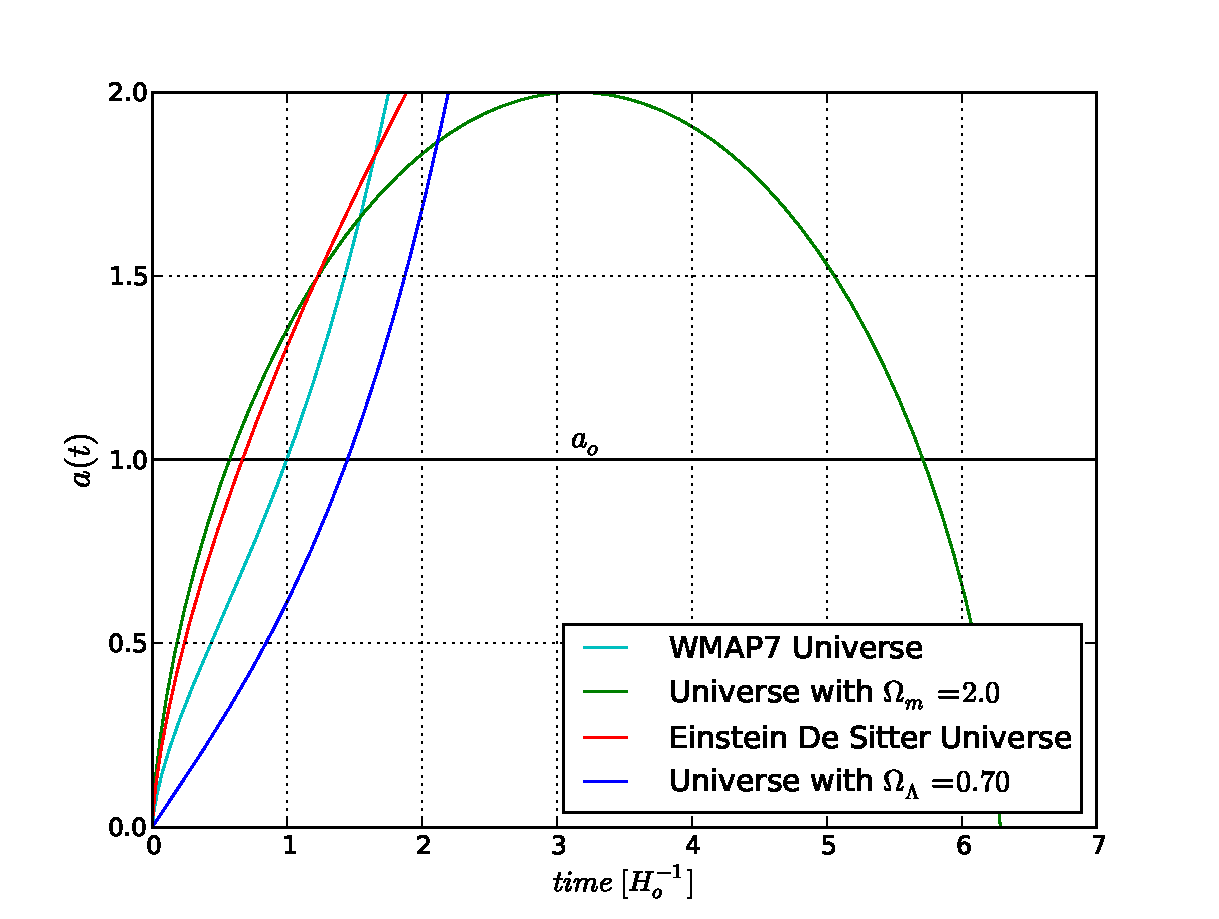
\includegraphics[width=0.8\textwidth]{Images/chapter2/factordeescala.pdf}
       \caption{ \small Scale factor as a time function. The Universe expansion for 
       different density contributions. A closed Universe is obtained when 
       $\Omega_m = \Omega_o>1$. Also, the PLANCK parameters show an accelerated expansion. 
        }
       \label{factor}
 \end{figure}
%**********************************************************************************************************************

%&&&&&&&&&&&&&&&&&&&&&&&&&&&&&&&&&&&&&&&&&&&&&&&&&&&&&&&&&&&&&&&&&&&&&&&&&&&&&&&&&&&&&&&&&&&&&&&&&&&&&&&&&&&&&&&&&&&&&&
\section{Hilbert-Einstein field equation}
%&&&&&&&&&&&&&&&&&&&&&&&&&&&&&&&&&&&&&&&&&&&&&&&&&&&&&&&&&&&&&&&&&&&&&&&&&&&&&&&&&&&&&&&&&&&&&&&&&&&&&&&&&&&&&&&&&&&&&&

At big scales, the most important fundamental interaction of nature is the 
gravitational one. Hence, the theory of general relativity (TGR) is 
an essential tool in the study of the cosmos. 
At smaller scales, the Newtonian gravitational theory might be used, where
the Poisson equation offers a relation between the second derivative of the
gravitational potential $\Phi$ and the source of the field $\rho$

\[ \nabla^2\Phi=4\pi G\rho\]

this equation is obtained from TGR for low velocities and 
a weak gravitational field ($\Phi/c^2<< 1$). A key equation of TGR is
the Hilbert-Einstein field equation, a 6 independent component tensorial 
equation

\begin{equation}
R_{\mu\nu}-\f{1}{2}g_{\mu\nu}R-g_{\mu\nu}\Lambda = \f{8\pi G}{c^4}T_{\mu\nu}
\label{HEE}
\end{equation}

in equation \ref{HEE} the first term of the left side is Ricci's tensor 
(second derivatives of the metric tensor). 
The second one contains the scalar of curvature $R$ that defines space-time geometry. 
In the third term, $\Lambda$ is the cosmological constant that could be associated with
the vacuum density term and is responsible for the accelerated expansion of the Universe.  

In the right side of the equation, the tensor energy-momentum $T_{\mu\nu}$ is present.
It includes, as its name suggest, all the contributions to energy and momentum. 

Hence, the left side of the equation has associated geometry terms, 
while the right one, the ones associated with the matter and energy distribution. 
Then, it could be interpreted as if geometry is determined by the matter-energy content 
of the Universe, though, strictly speaking, the energy-momentum tensor depends
in the metric tensor too. 

There is an interesting case of this tensor when we are dealing with a perfect 
fluid, i.e., without viscosity. It shows that not only density causes curvature of space-time 
but also pressure. The Universe can be modeled with this particular
shape of the energy-momentum tensor. It can be expressed as 

\[T^{\mu}_{\sigma}= diag\{c^2\rho,-P,-P,-P\}\]

where $\rho$ is the density and $P$ is the fluid pressure. 

\

There are several solutions to the Einstein field equation but not
many in an analytical form. An analytical solution is Schwarzchild's solution that 
represents the metric of a static spherical mass. Other possible solution is the Kerr 
metric that corresponds to a rotating uncharged mass. The Robertson
Walker metric satisfies these equations too. 
	

%&&&&&&&&&&&&&&&&&&&&&&&&&&&&&&&&&&&&&&&&&&&&&&&&&&&&&&&&&&&&&&&&&&&&&&&&&&&&&&&&&&&&&&&&&&&&&&&&&&&&&&&&&&&&&&&&&&&&&&
\section{ Friedmann equations }
%&&&&&&&&&&&&&&&&&&&&&&&&&&&&&&&&&&&&&&&&&&&&&&&&&&&&&&&&&&&&&&&&&&&&&&&&&&&&&&&&&&&&&&&&&&&&&&&&&&&&&&&&&&&&&&&&&&&&&&


From HE field equations and the RW metric it is possible to propose 
cosmological models that give account for the observed dynamics
in the Universe. In this direction, the components of the 
field equation can be taken, $\beta=\nu= 0$, time-time component,
and $ii=1,2,3$ (space-time components), from where one gets, for the scale
factor

\begin{equation}
\frac{\ddot{a}}{a} = -\frac{4\pi G}{3 }\left( \rho + 3 \f{P}{c^2} \right)+\frac{\Lambda c^2}{3} 
\label{fried1}
\end{equation}

\begin{equation}
\f{\ddot{a}}{a}+2\f{\dot{a}^2}{a^2}+2\f{c^2 K}{a^2} = 4\pi G\left( \rho-\frac{P}{c^2}\right)+\Lambda c^2
\label{fried2}
\end{equation}

\

where, it has been used the energy momentum tensor for an ideal fluid. 
The former expressions are the Friedmann equations and are written in a form
that can account for the Universe expansion. In equations \ref{fried1} and \ref{fried2}
$a(t)$ is the scale factor that is set to one for the actual epoch,
$a(t_o)=1$, $\rho$ is the total density (radiation plus matter density), $P$ is
the total pressure.  

The equation \ref{fried1} has the form of force equation and it can
be partially deduced from newtonian mechanics (without the pressure
and cosmological constant terms). A most convenient and used form
is obtained after algebraically manipulating them, a second form of 
FE that can be interpreted as an energy equation

\begin{equation}
H(t)=\frac{\dot{a}^2}{a^2}=\frac{8 \pi G}{3}\left(\rho+\frac{\Lambda c^2}{8\pi G}\right) -\frac{Kc^2}{a^2}
\label{fried3}
\end{equation}

where the first term in the right hand side is the potential energy. 
This equation also allows to define the Hubble parameter since $H(t)=\dot{a}^2/a^2$ and for the 
actual epoch its value is equal to $H(t_o)=H_o = 100h$ Km $s^{-1}$ $Mpc^{-1}$ where $h=0.6774$
according to Planck measures. 

Additionally \ref{fried3} can be expressed in terms of the critical
density, i.e. the matter-energy density required for a flat Universe.
%the matter-energy density necessary for the Universe to be flat. 
Therefore, if the Universe has a bigger density,
$\rho > \rho_{crit}$, it would collapse about itself. Conversely, the Universe would
continue to expand indefinitely. The critical density is defined as

\[\rho_{crit}(t)= 3H(t)^2/8\pi G\]

Dividing \ref{fried3} by the Hubble constant $H_o$ and defining 
the density parameter  $\Omega_{i,o} = \rho_{i,o}/\rho_{crit}(t_o)$ 
with $i=m,r,\Lambda$ is obtained the next expression, thus different 
contributions of the density to the Hubble parameter are observed, i.e., 
matter, radiation and vacuum density

\begin{equation}
\frac{H^2(z)}{H_o^{2}}=\Omega_{m,o}\left(1+z\right)^3+
\Omega_{r,o}\left(1+z\right)^4+ \Omega_{\Lambda,o} + ( 1-\Omega_o)
\left(1+z\right)
\label{fried4}
\end{equation}


where $\Omega_o=\Omega_{m,o} +\Omega_{r,o}+\Omega_{\Lambda,o}$ and
it has been introduced the relation between redshift and scale
factor $1+z=1/a$. Every term of matter-energy density 
is a different function of the Universe expansion, although the vacuum 
energy does not depend on the redshift, this is, is constant through time.

\

Initially the Universe was dominated by the radiation, during 
this epoch matter and radiation were coupled, i.e., the De Broglie 
electrons wavelenght were comparable to the wavelength of photons. Because
of this, collisions between photons and electrons were very frequent causing
that the mean free path of the photons be negligible and that the Universe 
would be opaque. 
During this coupling, radiation and matter had the same temperature
and its behavior is explained as a black body. 
As can be seen in the figure \ref{densidad}, from $z=3230$
matter becomes the major contribution to the Universe density.
When $z=1100$ the temperature drop is big enough and the
recombination rate turns higher than the ionization one. 
%Recombination refers to the formation of neutral atoms,
%that was the ultimate cause to decoupling. 
The last radiation dispersion due to matter still can be
observed, and it is called cosmic radiation background (CMB).
Because of the Universe expansion, its temperature
has been dropping, and it is nowadays around $T$ = $2.7K$. 
  
%**********************************************************************************************************************
\begin{figure}[htbp]
       \centering
               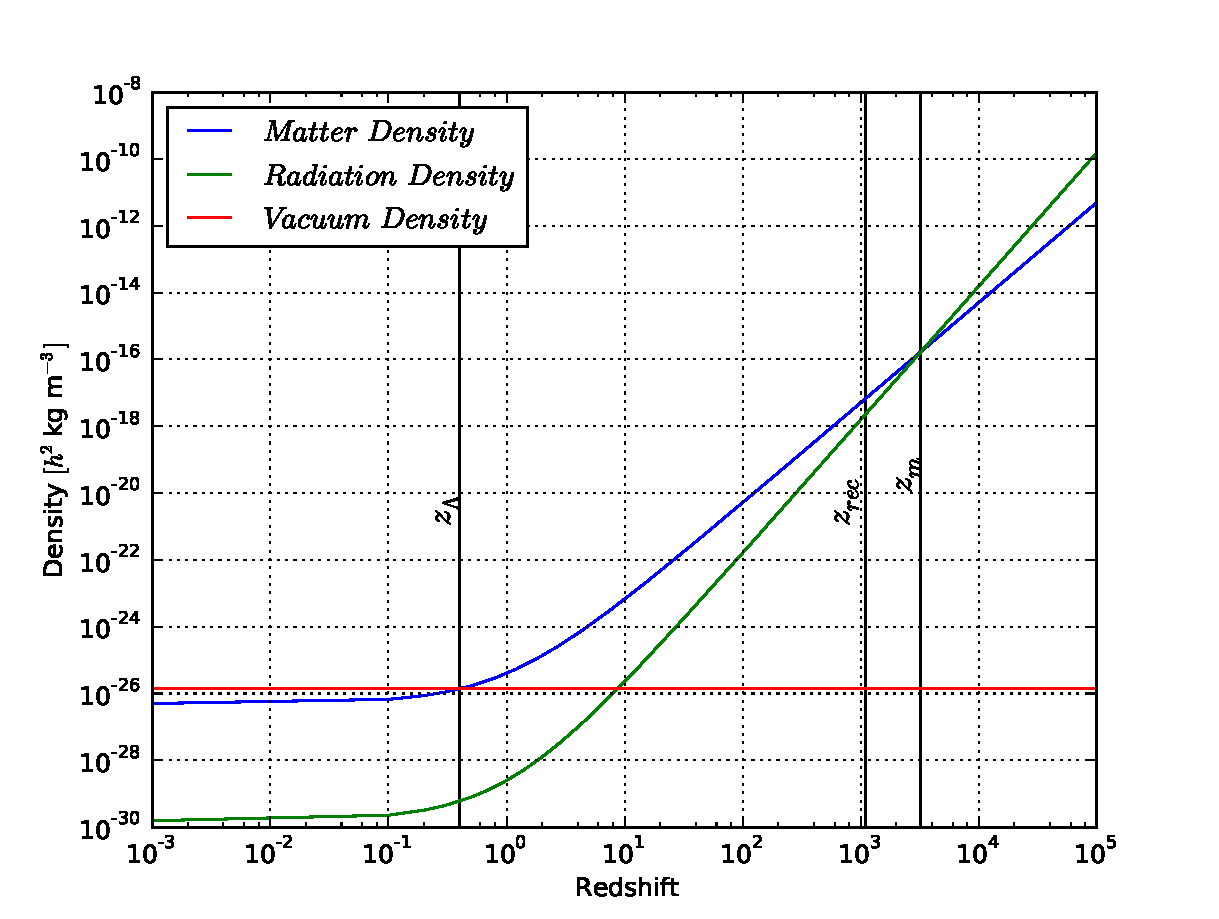
\includegraphics[width=0.8\textwidth]{Images/chapter2/density.pdf}
       \caption{ \small Dependence in redshift for $\Omega_\Lambda$, $\Omega_m$ and
       $\Omega_r$. The decoupling between matter and radiation is obtained when 
       $z_{rec}$.
        }
       \label{densidad}
 \end{figure}
%**********************************************************************************************************************

Nowadays, the dominant density component in the Universe is vacuum, $\rho_{\Lambda}$, 
though it is a constant since it does not depend on the scale factor, as already
stated. In contrast, matter depends on the scale factor as $a^{-3}$ and radiation as 
$a^{-4}$ causing both components diminish in time. 

The cosmological constant could be associated to vacuum energy that causes an
opposed behavior in the Universe dynamics compared to mass density, i.e., 
it accounts for the accelerated universe expansion. 

There are several solutions to \ref{fried3}, for instance in the Einstein de 
Sitter Universe, there are no radiation or vacuum contributions to the density
and the total density is $\Omega_o=1.0$. In this particular case, the solution
is

\[
t = \f{2}{3H_o}(1+z)^{-3/2}
\]

Therefore, depending on the chosen density values, the equation \ref{fried3}
has different solutions and one can expect several Universe models, i.e.,
depending on the parameters chosen, the Universe's evolution changes.  
In the case of Planck, the parameters used are shown in table \ref{plancktable}. 

\begin{table}
\begin{center}
  \begin{tabular}{ | c | c | c |}
    \hline \hline
    Parameter & Symbol & Best fit \\ \hline \hline 
    Hubble constant $(km/Mpc$-$s)$ & $H_0$ & 67.74$\pm$0.46 \\ \hline
    Baryon density & $\Omega_b h^2$ &  0.02230$\pm$0.00014 \\ \hline
    Cold dark matter density & $\Omega_c h^2$ & 0.1188$\pm$0.0010 \\  \hline
    Dark energy density & $\Omega_\Lambda$ & 0.6911$\pm$0.0062 \\ \hline
    Scalar spectral index & $n_s$ & 0.9667$\pm$0.0040 \\ \hline
    Sigma 8 & $\sigma_8$& 0.8159$\pm$0.0086 \\ \hline
  \end{tabular}
    \caption{ Fit cosmological parameters from Planck results\cite{planck}.}
  \label{plancktable}
\end{center}
\end{table}

Other possible Universe models are for example, one obtained when matter
density parameter is the only contribution to total universe density but 
it is bigger than 1. In such a case the Universe obtained is closed. 
Other one, it is one obtained when the Universe is dominated for the vacuum
contribution. In this case, the Universe is always open. When all the 
contributions are present, the Universe can be open or closed depending on the
total density parameter. 
		
%&&&&&&&&&&&&&&&&&&&&&&&&&&&&&&&&&&&&&&&&&&&&&&&&&&&&&&&&&&&&&&&&&&&&&&&&&&&&&&&&&&&&&&&&&&&&&&&&&&&&&&&&&&&&&&&&&&&&&&
\section{ Equation of state }
%&&&&&&&&&&&&&&&&&&&&&&&&&&&&&&&&&&&&&&&&&&&&&&&&&&&&&&&&&&&&&&&&&&&&&&&&&&&&&&&&&&&&&&&&&&&&&&&&&&&&&&&&&&&&&&&&&&&&&&

As mentioned before, scale factor characterizes the Universe expansion, 
then finding relations between each density component of the Universe 
with this factor is an important task. Below is shown only a relation of proportionality 
between them. For further details \cite{padma} is a good reference. 

\

\textbf{Matter density:} Assuming that all matter content in the Universe is an 
isolated system, the first law of thermodynamics is expressed as $dU = -pdV$, 
where relativistic terms are included in the internal energy term. 
Using the equipartition theorem and deriving the internal energy with respect to 
the scale factor is obtained

\[ T \propto a^{-2} \]

but from the equation of state $P = NkT$ and taking into account that $N = N_oa^{-3}$  

\begin{equation}
P \propto a^{-5}
\end{equation}


Pressure exerted by matter decreases strongly with Universe's expansion, while density 
and temperature changes are more slow. The latter is other cause in order that vacuum 
dominates the Universe expansion.

\

\textbf{Radiation density:} Radiation energy density expressed in terms of the 
photon density, $N(\nu)$, is 

\[\xi=\sum_{\nu}N(\nu)h\nu\]

where $N(\nu)$ satifies the relation $N \propto (1+z)^3$ and $\nu \propto (1+z)$ 
such that $\xi \propto a^{-4} $. Comparing the last result with Stefan-Boltzmann law 
one can concluded that 

\[T\propto a^{-1}\]
 
Finally, radiation pressure dependence on scale factor is found with the equation 
$ P=\epsilon_{total}/3$, so

\begin{equation}
P \propto a^{-4}
\end{equation}
\

\textbf{Vacuum density:} On the other hand, vacuum satisfies $\epsilon {total}=\rho c^2$ 
where $\rho$ is an effective density. Replacing this result in the first law of thermodynamics
and deriving with respect to scale factor

\begin{equation}
 P=-\rho c^2 = -\f{ \Lambda c^4}{8\pi G}
\end{equation}

the vacuum density constancy is used for the deduction of the latter expression.

%&&&&&&&&&&&&&&&&&&&&&&&&&&&&&&&&&&&&&&&&&&&&&&&&&&&&&&&&&&&&&&&&&&&&&&&&&&&&&&&&&&&&&&&&&&&&&&&&&&&&&&&&&&&&&&&&&&&&&&
\section{ Perturbation evolution in the newtonian regime }
%&&&&&&&&&&&&&&&&&&&&&&&&&&&&&&&&&&&&&&&&&&&&&&&&&&&&&&&&&&&&&&&&&&&&&&&&&&&&&&&&&&&&&&&&&&&&&&&&&&&&&&&&&&&&&&&&&&&&&&

As already stated, there is no radiation comming toward us from a previous 
epoch to decoupling. Although, due to the last scattering between radiation
and matter, highly homogeneous and isotropic distribution of matter is
inferred from the patterns obtained from background cosmic radiation\footnote{
Image taken from \url{http://www.esa.int/spaceinimages/Images/2013/03/Planck_CMB}} 
as shown in Figure \ref{CMB}.

In the CMB radiation, small temperature perturbations are observed indicating 
the presence of small matter perturbations at this epoch. These are the initial 
seeds from where structures observed nowadays formed. 

%At the present time the wavelength associated to this cosmic radiation is in the 
%microwave range.

In this structure growth, density perturbations are increasing but it is not
until they got a size of $\delta\sim 1$ that this growth is dominated by gravity. 
The perturbations have grown enough to start talking 
about galaxy formation when their density gets around $1\times 10^6$ compared to
the background density, this happens for a epoch around $z\sim 100$ for halos with gas 
that have cooled enough.

But, it is still important to study the initial stages of the perturbations.
Because of this, a linear regime treatment for perturbations when $\delta\ll 1$
are key in such a study. 

%**********************************************************************************************************************
\begin{figure}[htbp]
       \centering
               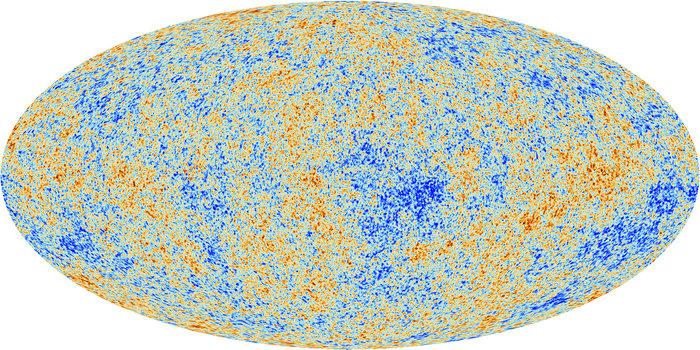
\includegraphics[width=0.6\textwidth]{Images/chapter2/Planck.jpg}
       \caption{\small Cosmic background radiation image obtained by Planck satellite.}
       \label{CMB}
 \end{figure}
%**********************************************************************************************************************


%######################################################################################################################
\subsection{ Newtonian description  }
%######################################################################################################################


Inflation is an exponential expansion of the space-time in the initial stages of the 
Universe. In this stage quantum perturbations were magnified to cosmic size, forming 
inhomogeneities of the density field, the seeds for the large scale structure of the Universe. 
Here, the initial density perturbations considered have a characteristic length much smaller 
such that the relativistic effects can be neglected, i.e., perturbations do not affect the local
metric. 
%This implies that the size of the perturbations is very small compared with scales where the Universe curvature  is significant, making this Newtonian approximation be valid. Because of this, causality  is taken as granted.

In this Newtonian approximation the equations of gas dynamics for a fluid in a gravitational
field can be considered. For a fluid in motion with a velocity distribution $\textbf{u}$ and 
density $\rho$ subject to a gravitational $\phi$ field that suffers changes in its pressure $P$ 
satisfies 

\begin{eqnarray}
\der{\rho}{t}&=& -\rho \nabla_r\cdot \textbf{u} \nonumber\\
\der{\textbf{u}}{t} &=& -\f{\nabla_r P}{\rho}-\nabla_r\phi \nonumber\\
\nabla_r^2 \phi & =& 4\pi G\rho 
\label{euler}
\end{eqnarray}

where an Eulerian description is used, i.e., the partial derivatives in the 
expressions \ref{euler} describe the variations of the properties at a fixed 
point in space, $r$ is the proper coordinate. 

Since density perturbations are the ones that trigger potential wells, they are 
more of our interest than the density field itself.
Then, it is useful to express the density as $\rho = \overline{\rho}(1 + \delta)$, where
$\overline{\rho}$ is the background density and $\delta$ is the overdensity of interest. 


Additionally, it is necessary to make clear another point. The velocity of the particles have 
two different contributions, the first one is because of the Universe expansion and 
the other one is the proper velocity of the particle, recessional 
and peculiar velocities respectively. 
From the latter mentioned, the coordinate system can be changed from \ref{euler}
an Euler description to a Lagrangian one, i.e., moving with the Universe expansion.
Let us see this in more detail, velocity in an Eulearian description is 
$\textbf{u}= a\dot{\textbf{x}}+ \textbf{x}\dot{a} = \textbf{v}+\textbf{x}\dot{a}$, 
where $\textbf{v}$ is the peculiar velocity and $\textbf{x}\dot{a}$ is the Universe 
expansion velocity. 
Then, transforming in comoving coordinates, coordinates that move with the Universe
expansion, and changing the density $\rho$ to density perturbations $\delta$, the equations 
\ref{euler} can be written as 

\begin{eqnarray}
\pder{\delta}{t} &=& -\f{1}{a}\nabla\cdot[(1+\delta)\textbf{v}]\nonumber\\
\pder{\textbf{v}}{t}+\f{\dot{a}}{a}\textbf{v}+\frac{1}{a}(\textbf{v}\cdot\nabla)\textbf{v}& = &
-\f{\nabla \Phi}{a}-\f{\nabla P}{a\overline{\rho}(1+\delta)}\nonumber\\
\nabla^2 \Phi &=& 4\pi G\overline{\rho}a^2\delta
\label{ec.movimiento}
\end{eqnarray}

the first equation corresponds to the continuity equation, the second one is Euler's 
equation and the last one is Poissonian gravitational field equation with $\Phi = \phi +a\ddot{a}x^2/2$. Velocity components appear due to gravitational interactions and changes in pressure.

\

Additionally, equation of state relating the thermodynamic quantities pressure P, 
density $\rho$ and entropy $s$ for this cosmological fluid is 

\begin{equation}
P(\rho,s)= \left[\f{h^2}{2\pi(\mu m_p)^{5/3}}e^{-5/3}\right]\rho^{5/3}\exp \left(\frac{2}{3}\f{\mu m_ps}{k_B}\right)
\label{ec.estado}
\end{equation}

Manipulating algebraically the continuity equation, Poisson equation and state equation,
a wave equation for density perturbations can be obtained

\begin{equation}
\f{\partial^2\delta}{\partial t^2}+2\f{\dot{a}}{a}\pder{\delta}{t} =
4\pi G \overline{\rho}\delta + \f{C_s^2}{a^2}\nabla^2\delta+\f{2}{3}\f{\overline{T}}{a^2}\nabla^2s
\label{onda}
\end{equation}

where $\overline{T}$ is the background temperature and $C_s$ is the speed of sound.
The Universe expansion is seen in the second term in the left hand side. Since for an expanding
Universe the term $\dot{a}/{a}$ is positive, its effect opposes to the 
perturbation growth. This result was expected since the expansion is against collapse leading to a decrease in growth. 	

The right hand side shows the causes for the evolution of the density perturbations. 
Entropy can be considered as the heat interchange between the perturbation and 
its surroundings, causing the expansion or growth of the perturbation. As expected, 
gravitational field is a source for perturbation growth. 

A solution to the perturbation equation in terms of Fourier series is proposed as

\begin{eqnarray}
\delta(x,t) &=& \sum_k \delta_k(t)e^{ik\cdot x} \nonumber\\
s(x,t) &=& \sum_k s(t)e^{ik\cdot x} \nonumber
\end{eqnarray}

where $\textbf{k}$ is the wave number and $\delta_k$ is 
a density mode that can be calculated using the discrete Fourier transform
of the density field. Hence, every mode depends on all known values
of the density perturbations. 

An important aspect in the last expression is the independence of the 
functions $e^{ik\cdot x}$ allowing equation \ref{onda} to be expressed as 

\begin{equation}
\f{d^2\delta_k(t)}{dt^2}+2\f{\dot{a}}{a}\der{\delta_k(t)}{t} = 
\left[4\pi G\overline{\rho}-\f{C_s^2 k^2}{a^2}\right]\delta_k(t)
-\f{2}{3}\f{\overline{T}}{a^2}k^2s_k(t)
\label{ec.modos}
\end{equation}

the solution of this equation provides expansion coefficients for the Fourier series,
from where, the behavio	r of density perturbations, their growth or 
dissipation, is obtained. 

%######################################################################################################################
\subsection{ Jeans Inestability}
%######################################################################################################################

Before solving equation \ref{ec.modos}, it is important to develop
some intuition about the	 physical phenomena. This can be achived making some 
simplifications, for example, taking an isentropic static Universe ($\dot{a}=0$)
the expression becomes

\[
\f{d^2\delta_k(t)}{dt^2} + \omega^2\delta_k(t) = 0
\]

with $\omega^2 = C_s^2k^2/a^2-4\pi G\overline{\rho}$. Now, let us analyse
the different solutions of the previous expression. When the relation 
$C_s^2k^2/a^2>4\pi G\overline{\rho}$ is satisfied the frequency $\omega$ is
possitive. The solution represents a sound wave, an oscillatory solution where 
gravity instabilities are contrarrested by radiation pressure. Thus, this 
particular solution is not of our interest, matter is not going to agglomerate due 
to gravity. 
On the other hand, if $4\pi G\overline{\rho}>C_s^2k^2/a^2$ the solution takes the form 
$\delta_k(t)\propto e^{\Gamma_k t}$, where $\Gamma_k=i\omega_k$ is the growth rate. 
Hence, the density mode can grow or dissipate depending on the growth rate, a negative 
rate causes dissipation but a positive one produces a gravitational collapse.

%Clearly the solution of equation \ref{ec.modos} depends on $\omega$'s sign. If $C_s^2k^2/a^2>4\pi G\overline{\rho}$,  $\omega$ is positive, in this case the solution is oscillatory one. this solution represents a sound wave, then this density mode is not going to agglomerate because of gravitational instabilities, therefore it is not of our interest. 
%By the other side, if $4\pi G\overline{\rho}>C_s^2k^2/a^2$ the solution takesthe form $\delta_k(t)\propto e^{\Gamma_k t}$, with $\Gamma_k=i\omega_k$ named growth rate. In this case, the perturbation dissipates or collapses dependingon the square frequency sign chose. 
Concluding, density modes tend to collapse because of gravitational instabilities but 
pressure gradients appear due to atomic interactions causing dissipation. Then, both 
components must be considered. 
But the perturbations that collapse are the subject of our study. 


For this, a minimum length that a perturbation must have to obtain an 
inestable fluctuation, i.e., a collapsing
perturbation, is defined. Hence, from the frequency Jeans' length
is obtained $\lambda_J = 2\pi a/k_j$ and satisfies 
$\lambda_J = 2\pi/k_j = C_s(\pi/G\rho)^{1/2}$.
The growth rate can be rewritten in terms of $\lambda_J$, 
allowing to make the next comparison, if $\lambda_{pert}>>\lambda_J$
is satisfied the perturbation collapses, here $\lambda_{pert}$
is the length of the perturbation.

As was shown previously, Jeans' length depends on the speed of sound
that is defined as 

\[
C_s^2 = \left( \pder{P}{\rho} \right)_s
\]

and using also the equation of state \ref{ec.estado} a relation 
is found. It was also used the fact that radiation and matter 
temperature are equal for $z \leq z_{eqv}$ due to coupling. 
But after decoupling every component evolves independently. 
Jean's length and mass, the last one defined as $M_J =  \pi\overline{\rho}_{m,o}\lambda_J^3 $,
are given by

\begin{eqnarray}
\lambda_J \approx 0.01(\Omega_{b,o}h^2)^{-1/2}Mpc\\
M_J \approx 1.5\times 10^5 (\Omega_{b,o}h^2)^{-1/2}M_{\odot}
\end{eqnarray}

Before decoupling, speed of sound was affected not only 
by matter but for radiation, even the latter one was more
important since radiation density dominates in this epoch
(figure \ref{densidad}). 
The valid state equation for radiation in this epoch is
$P = c^2\rho_r/3$ and it can be shown that the change 
in magnitude order evaluated before and after decoupling
of Jean's length and mass is $2.6\times 10^{-5}$ and $1.8\times 10^{-14}$
respectively. From previous asseveration a possible conclusion is
decoupling increases gravitational collapse since  minimum characteristic length
required for collapsing becomes smaller. 

\

Until now dark matter has not been mentioned, a component that contrary
to baryonic matter does not interact with radiation. But it is around
$23\%$ of the overall Universe content, making it responsible for the 
large scale mass distribution observed. Dark matter particles interact
among them and with baryonic matter through gravitational interaction.
This leads to dark matter potential wells where baryonic matter can also fall.  
It occurs around $z \sim 3500$. But, dark matter initial seeds for potential 
wells are formed before decoupling, since they do not interact with radiation,
they can gather forming them. While this happens, baryonic matter and radiation 
interacts gravitationally with dark matter, leading to no formation of 
baryonic seeds precisely because of the mentioned coupling. Later a more detailed 
explanation will be provided. 

The last arguments exposed allow to express perturbations as $\delta = \delta_oD(z)$,
where $\delta_o$ is an initial seed from where a dark matter potential well formed
and $D(z)$ is a growing function of an initial seed.
Then, rewritting equation \ref{ec.modos}  

\[
\f{d^2D(z)}{dz^2}+\left[ \f{H'(z)}{H(z)} -\f{1}{1+z}\right]\der{D}{z}
= \f{1}{H^2(z)}\left[ \f{4\pi G\overline{\rho}(z)}{(1+z)^2} \right]D(z)
\]

%**********************************************************************************************************************
\begin{figure}[htbp]
       \centering
               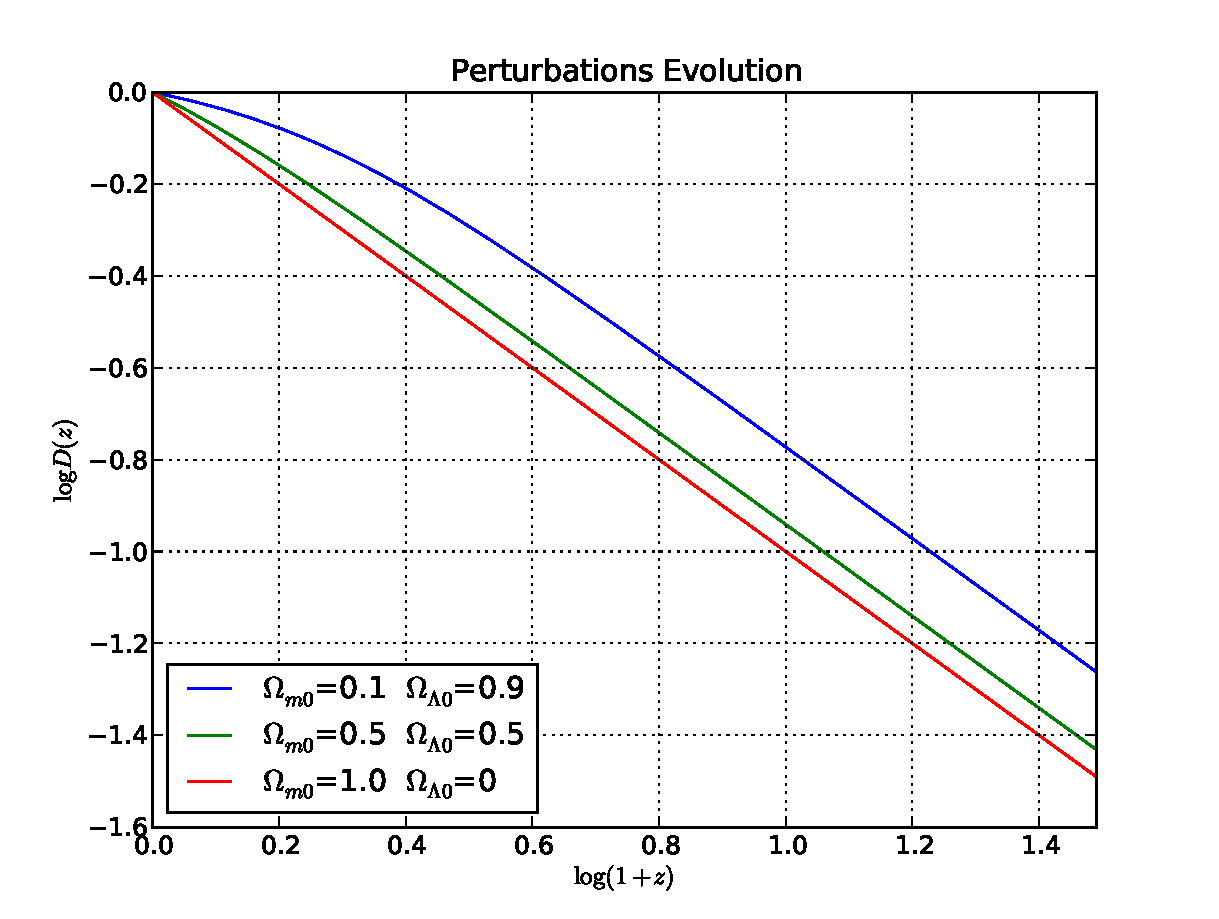
\includegraphics[width=0.8\textwidth]{Images/chapter2/masavacio.pdf}
       \caption{\small Perturbation evolution for a model Mass-vacuum, the behaviour
       for different contributions of each component. }
       \label{masavacio}
 \end{figure}
%**********************************************************************************************************************

in the expresion isotropy was assumed and the velocity term was neglected
since the perturbations of our interest satify $\lambda_J \ll \lambda$.
Using the last equation, different solutions changing density parameters
are obtained. For example, an Einstein de Sitter Universe  $\delta_k(z)=\delta_o(1+z)^{-1}$,  
an Universe dominated by radiation $\delta_k(z)=\delta_o(1+z)^{-1.22}$ and
an Universe dominated by vacuum $\delta_k(z)=\delta_o(1+z)^{-0.58}$. 
Obviously, for different contributions to every component of density can be found,
in figure \ref{masavacio} is shown perturbations evolution for a model with
matter and vacuum contributions. As expected, for bigger matter density
perturbations grow faster while for universes with bigger vacuum contribution, 
perturbations grow slower cause accelerated expansion. In the latter, a bigger
initial mass is required to start collapsing. In the figure, largest redshift
is $z=0$ but solution is only valid while $\delta\ll 1$. 

%&&&&&&&&&&&&&&&&&&&&&&&&&&&&&&&&&&&&&&&&&&&&&&&&&&&&&&&&&&&&&&&&&&&&&&&&&&&&&&&&&&&&&&&&&&&&&&&&&&&&&&&&&&&&&&&&&&&&&&
\section{ Higher order perturbation theory }
%&&&&&&&&&&&&&&&&&&&&&&&&&&&&&&&&&&&&&&&&&&&&&&&&&&&&&&&&&&&&&&&&&&&&&&&&&&&&&&&&&&&&&&&&&&&&&&&&&&&&&&&&&&&&&&&&&&&&&&

As mentioned, perturbations start growing after decoupling. This growth leads
precisely to an increase in their density contrasts. 
When they have increased enough, around $\delta\sim 1$, Newtonian description 
stops being valid. A first approach to study such perturbations is spherical collapse. 
Even for those $\delta$ values, perturbations are not considered an object. 
In such cases, gravitational interaction determines dynamics more than Universe
expansion. This ocurrs when density gets around $\sim 100 \overline{\rho}$. 

Now, let's see in more detail spherical collapse. In this scenario a perturbation
has spherical symmetry and pressure exerted among particles is neglectable. 
But the latter supposition would imply that collapsing cause perturbations 
to end up as a singularity, since there is no force against collapse.
If tidal forces are included it would not be the case but it is taken 
as a first approximation.

Time calculated for a perturbation to collapse is 

\[
1+z_c = \f{1+z_{max}}{2^{2/3}}
\]

where $z_{max}$ is redshift when perturbation dynamics is no longer affected by Universe
expansion. Collapsing time for a perturbation is smaller than time necessary to become 
a gravitationally linked object. Aditionally redshift estimative for a perturbation
satisfies virial theorem is

\[
(1+z_{vir})\leq 0.47\left( \f{v}{100kms^{-1}}\right)^2\left( \f{M}{10^{12}M_{\odot}}\right)^{-2/3}(\Omega_oh^2)^{-1/3}
\]

it can be noticed from this expresssion that more masive objects and with a bigger 
dispersion velocity have a bigger viralization time. 

%######################################################################################################################
\subsection{ Zeldovich approximation }
%######################################################################################################################

The last model for a non lineal perturbartion treatment 
has several failures. A next step in this direction is 
Zeldovich approximation that provides a more realistic description, 
since it considers that perturbations' shape is an ellipsoid.
Though pressureless and without viscosity fluid supposition are still taken.
Coomovil coordinates satisfies 

\[
\textbf{x} = a(t)\textbf{r}+b(t)\textbf{p}(\textbf{r})
\]

where $\textbf{r}$ are Eulerian coordinates and $b(t)\textbf{p}(\textbf{r})$
is the displacement respect to the initial position. The last term is related 
with the gravitational potential generated by initial perturbations. 
It can be shown that initial perturbations are given by 

\[
\rho = \frac{\overline{\rho} }{[1-\alpha b(t)][a(t)-\beta b(t)][a(t)-\gamma b(t)]}a^3(t)
\]

where $\alpha$, $\beta$ and $\gamma$ account for the expansion or contraction 
along the three main axis of the ellipsoid. 
When  $\alpha \geq \beta \geq \gamma$ and $b(t)$ are sufficiently big enough a 
singularity appears. If $\alpha$ also gets its highest value causes that perturbations
get a pancake shape due to a faster contraction in x axis. 
Despite of the simplicity, it is a model accurate with numerical results. Hence,
it is used in observational cosmology and initial condition generation in N body
simulations. 

%&&&&&&&&&&&&&&&&&&&&&&&&&&&&&&&&&&&&&&&&&&&&&&&&&&&&&&&&&&&&&&&&&&&&&&&&&&&&&&&&&&&&&&&&&&&&&&&&&&&&&&&&&&&&&&&&&&&&&&
\section{ Statistical properties of cosmological perturbations }
%&&&&&&&&&&&&&&&&&&&&&&&&&&&&&&&&&&&&&&&&&&&&&&&&&&&&&&&&&&&&&&&&&&&&&&&&&&&&&&&&&&&&&&&&&&&&&&&&&&&&&&&&&&&&&&&&&&&&&&

Nevertheless, to study the evolution of the Universe since decoupling requiere to know 
or assume a density field, to know density in every point and its evolution with time. 
But using the concept of density contrast $\delta = (\rho - \overline{\rho})/\overline{\rho}$, 
leads to a density perturbation field, which is a clearer way to analyse the evolution
of the density field.

In linear regime, there are a huge amount of perturbations described by different 
fourier modes. Since they evolve independently their amplitudes change with time and 
can be modelled using a transfer function $T(k)$ and a linear growth rate $D(t)$. 
To characterize such amount of density field values, statistical 
properties must be defined. 
This is, not considering individual positions or properties but instead moments defined from
some distribution function. This idea is supported by the fact that there is no access 
to the primordial perturbations that originated the large scale structure observed 
nowadays. Hence, our Universe could be considered as a realization of a random process 
where a statistical treatment results as a natural way to study it. 

Consider that the Universe can be divided into small cells, each of them with position 
$x_i$. These can be statistically characterized with a joint probability 
distribution and its moments that, in principle infinite, would describe the 
cosmic density perturbation field. 
Following this approach, the probability of having a mode between $\delta_k$ and 
$\delta_{k}+d\delta_k$ is, 

\begin{equation}
\mathcal{P}(\delta_{\mbox{\boldmath$\kappa$}})r_{\mbox{\boldmath$\kappa$}}dr_{\mbox{\boldmath$\kappa$}}d\phi_{\mbox{\boldmath$\kappa$}}
=
\exp\left[-\f{r_{\mbox{\boldmath$\kappa$}}^2}{2V_u^{-1}P(\kappa)}\right]	\f{r_{\mbox{\boldmath$\kappa$}}}{V_u^{-1}}
\f{dr_{\mbox{\boldmath$\kappa$}}}{P(\kappa)}\f{d\phi_{\mbox{\boldmath$\kappa$}}}{2\pi}
\label{probabilidad}
\end{equation}


where $r_{\mbox{\boldmath$\kappa$}}$ corresponds to perturbations amplitude,  $\phi_{\mbox{\boldmath$\kappa$}}$ 
is the phase and varies between $[0,2\pi)$. The joint probability distribution function 
is useful because it allows the independence of the terms $\delta_{\mbox{\boldmath$\kappa$}}$, 
or in other words it is the product of every mode

\[
\mathcal{P}_{\mbox{\boldmath$\kappa$}}(\delta_{\mbox{\boldmath$\kappa$}1},...,\delta_{\mbox{\boldmath$\kappa$}N})=
\prod_{\mbox{\boldmath$\kappa$}}\mathcal{P}_{\mbox{\boldmath$\kappa$}}(\delta_{\mbox{\boldmath$\kappa$}})
\]


This expression is not satisfied when the inverse fourier transform is done, since the 
probability density is not separable in the initial coordinate space. The term $P(\kappa)$ 
(assuming isotropy in \mbox{\boldmath$\kappa$}) is the power spectrum defined in the 
fourier space and it is related to the 2 point correlation function in the real space

\begin{equation}
P(k) = \f{4\pi}{V_u}\int_0^\infty \xi (r)\f{sin(kr)}{kr}r^2dr =  \langle|\delta(\mbox{\boldmath$\kappa$})|^2\rangle
\label{pk}
\end{equation}

as it can be seen in the expression, the isotropy of the universe is taken into account since during the power spectrum calculation, an average is done over all  possible orientations of the vector ${\mbox{\boldmath$\kappa$}}$

Here, $\xi (r)$  describes the distribution of points, telling for example, how clumpy certain region is or in general the clustering properties of the system. Being more specific, this function describes the excess probability of finding a particle at a distance $r$ from a particle selected at random over the expected in an uniform, random distribution. 
The two point correlation is defined as 

\[\xi (r) =  \langle  \delta(\textbf{x})\delta(\textbf{x}+\textbf{r}) \rangle\]

therefore, the density field leads to a direct way to find the power spectrum through a fourier 
transform. $\xi$ only depends on the amplitude of r because of the assumption of homogeneity
and isotropy, i.e., depends on relative distances. 

No clustering would imply that $\xi(r)$ is zero. A natural way to see this is through
a conditional probability, given that there is a particle in a volume element $dV_1$
the probability there is other one in a volume element $dV_2$ at a distance $r$

\[dP(2|1) = n[1+\xi(x_{12})]dV_2\]

if $\xi(x_{12})>0$ the probability of finding such pair of particles increases,
i.e., there is clustering of structures. But if $\xi(x_{12})<0$ such probability 
diminishes leading to an anticorrelation.  In the case where $\xi(x_{12})=0$ 
there would be no clustering, the distribution of particles would be the one of 
a random catalogue. 

Also, the function $\xi(r)$ can be expressed as a power law of the form

\[ \xi(r) = \left( \frac{r}{r_0} \right)^{-\Gamma} \]

being valid in the range $100 h^{-1}$ kpc to $10h^{-1}$ Mpc. The preferred
scale $r_0=5h^{-1}$ Mpc is the one where the galaxy density is greater than twice 
of the background. The exponent value is $\Gamma = 1.8$. This fit overestimates
the correlation function for distances bigger than $20 h^{-1}$ Mpc.  


\
 
So far, it has been shown two statistical measures, a fourier pair, in real space the 
correlation function and in fourier space the power spectrum. 
But other moments can be specified as previously mentioned, in general an l point 
correlation function can be defined through the next expression 
$\xi^l(\vec{x}_1,\vec{x}_2,\ldots \vec{x}_l) \equiv  \langle  \delta_1\delta_2 \ldots\delta_l)\rangle $ where the connected terms are the ones that contributed to the calculation.
For example, the first moment of the distribution is $\langle \delta(x) \rangle = 0$ because 
of the definition of density perturbation field. 

An important remark is that if initial density pertubations follow a gaussian distribution 
all moments higher than two (2 point correlation function) are zero, i.e., the density
perturbation field is completely described by the two first moments of the distribution. 

\

%**********************************************************************************************************************
\begin{figure}[htbp]
       \centering
               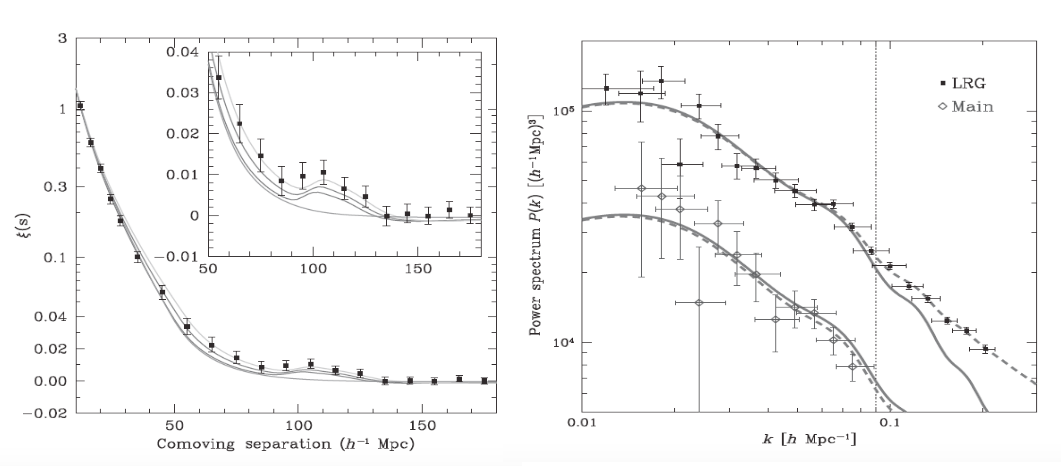
\includegraphics[width=0.95\textwidth]{./Images/chapter2/PS_CF.png}
       \caption{\small BAO peak in the correlation function in the left and the oscillations of BAO in the power spectrum in the right,
       (\cite{PLOT}).  
       The lower curve is the main SDSS sample and the upper one is the LGR sample. }
       \label{ps_cf}
 \end{figure}
%**********************************************************************************************************************

It is usually considered for the initial density field, that density contrasts 
follow a normal distribution centered in $\langle \delta \rangle = 0$. This idea is supported by
inflationary scenarios where a random gaussian perturbation field arises naturally from quantum 
perturbations during inflation, i.e., statistical behaviour lies on quantum perturbations. 
Since there are a large number of modes, the central limit theory 
would support this idea if the mode phases are independent. 
One of the advantages of this model is that the perturbation field remains gaussian during linear evolution. 

Additionally it has been found that the initial power spectrum expected from inflation theories 
has the form $P(\kappa)= k^n$. If $n=1$ the power spectrum is called Harrison-Zeldovich which is 
commonly used. 

With the initial power spectrum it can be done an inverse fourier transform and this way creating the initial density field. 

\

Furthermore, using inflationary models the shape of the linear power spectrum is well 
determined but there are not amplitude predictions, i.e., there is not a defined 
normalization of the power spectrum. 
One commonly way to do such thing is through the variance of the galaxy distribution when
sampled with randomly placed spheres at radius R. The relation between the variance of the 
density field and the power spectrum is

\[
\sigma^2(R) = \f{1}{2\pi^2} \int P(k)\hat{\omega}_R(k)^2k^2 dk
\]

where $\hat{\omega}_R(k)$ is the Fourier transform of the spherical top hot model.

\[\hat{\omega}_R(k) = \frac{3}{(k R)^2}[\sin(kR)-kR\cos(k R)]\]
 
In this approach $\sigma(R)$ is taken around one when $R=8h^{-1}Mpc$ because of 
measures performed observationally. 
Then, normalizing the power spectrum would imply to force $\sigma(R)$ to be one 
for the mentioned distance.

But several problems arise, one is that this normalization is not precisely valid
for linear regime since $\sigma(R)\approx 1$ when $\delta(R)\ll 1$. Other one is
baryonic matter is probably a bias tracer of the mass distribution. 

\

It is necessary to consider that after recombination epoch, density perturbations started
growing in size causing a non linear growth to appear. This implies a change in the 
density field and likewise the power spectrum. 



%######################################################################################################################
%\subsection{ Clustering in the real and redshift space }
%######################################################################################################################


%-----------------------------------------------------------------------------------------------------------
%\subsubsection{ Redshift distortions }
%-----------------------------------------------------------------------------------------------------------
%-----------------------------------------------------------------------------------------------------------
%\subsubsection{ Real space correlation functions }
%-----------------------------------------------------------------------------------------------------------

%&&&&&&&&&&&&&&&&&&&&&&&&&&&&&&&&&&&&&&&&&&&&&&&&&&&&&&&&&&&&&&&&&&&&&&&&&&&&&&&&&&&&&&&&&&&&&&&&&&&&&&&&&&&&&&&&&&&&&&
\section{ Baryonic acoustic oscillations }
%&&&&&&&&&&&&&&&&&&&&&&&&&&&&&&&&&&&&&&&&&&&&&&&&&&&&&&&&&&&&&&&&&&&&&&&&&&&&&&&&&&&&&&&&&&&&&&&&&&&&&&&&&&&&&&&&&&&&&&

Let us consider the epoch before recombination. The baryonic plasma (ionized protons and electrons) was coupled with radiation via 
Thomson scattering,  i.e., the electric field of photons accelerate charged particles making small density perturbations to disperse. Nevertheless,
considering that dark matter do not interact with radiation, small dark matter density contrasts can form. Hence, the baryons are 
subject to two competing forces, radiation pressure and gravitation. Consider a particular dark matter density contrast that attract
nearby baryons, they start clustering around the dark matter forming a bigger density contrast. But, due to the pressure caused
by coupling, the outward force becomes bigger than gravity, making baryons to move outward as a sound wave. This oscillation 
of the baryonic plasma is known as baryonic acoustic oscillation. 

\

When decoupling occurs and temperature drops, the force responsible for the expansion of the shell disappear, this is, 
the pressure caused by the coupling between baryons and radiation, leading baryons in the last position they were located. 
The scale of the baryonic acoustic oscillation is 
usually called the sound horizon and it can be computed as

\[  
s = \int_{z_{rec}}^{\infty} \f{c_s dz}{H(z)}
\]


where $c_s$ is the velocity of the propagation and $H(z)$ is the hubble param, (\cite{pilar}). 

Therefore, there is a spherical shell formed 
around the dark matter density perturbation. Now, not only dark matter density contrast seed gravitational instability but the baryons in the shell as well. 

The structures continue to grow reaching non linear growth and wipe out the imprint lead by the baryonic acoustic oscillations except for the bigger ones. The estimated size of the remaining BAO is $150$ Mpc, causing that scale to 
be more likely to have galaxy formation activity. The reason this distribution is not observed at cosmological scales is because
of the amount of imprints, they smear out the preferred scale. Though, it is expected an enhancement in the two point
correlation at scales of the baryonic oscillations. As was seen before, there is a direct correspondence between the 
two point correlation and the power spectrum. Hence, a characteristic oscillation in the power spectrum caused by the imprint of BAO is naturally found. 	

 
%**********************************************************************************************************************
\begin{figure}[htbp]
       \centering
               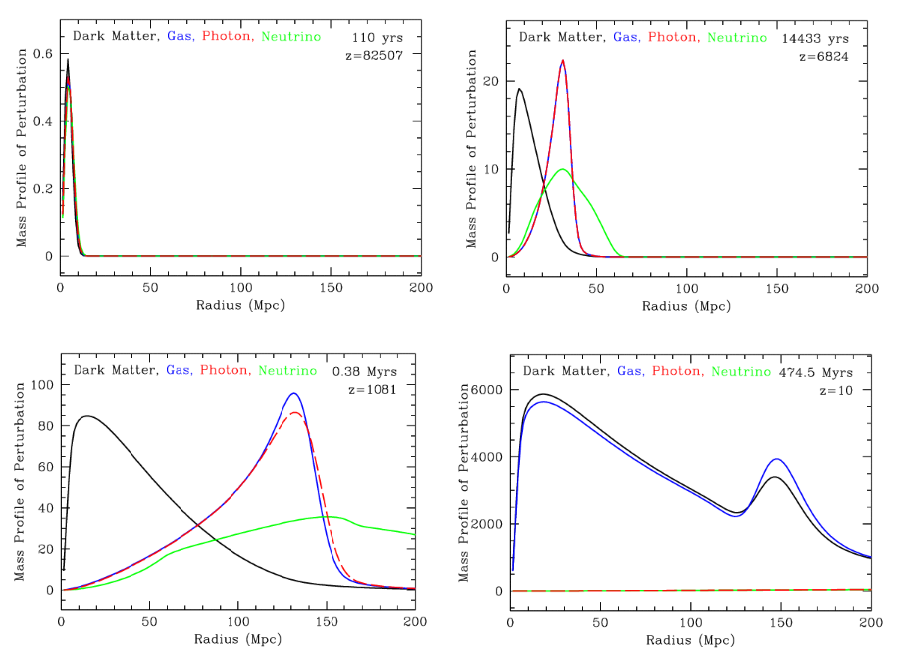
\includegraphics[width=1.0\textwidth]{Images/chapter2/BAOS2.png}
       \caption{\small All the figures show the evolution of the radial mass profile of dark matter,  baryons, photons
       and neutrinos. First one: Initial perturbations of the four species. 
       Second one: the neutrinos do not interact and move away, 
       the plasma of baryons and radiation overdensity expands because of radiation pressure, the dark matter
       continues to fall in the perturbation. Third one: The temperature drops enought to lead to decoupling, 
      the baryons slows down until stopped, the radiation and neutrinos continue moving away. Fourth one:  
      The dark matter and baryons eventually get the same distribution because of the gravitational interaction.}
       \label{DBM}
 \end{figure}
%**********************************************************************************************************************

Since baryonic acoustic oscillations are primarily a linear phenomenon, they are preserved in the power spectrum despite of 
the temporal evolution. Then,  BAO are used as an standard ruler, specifically for high redshift where other rulers tend to fail. 
This is commonly used for constraining dark matter models. 

\

Although, the nonlinear collapse change the shape and position of baryonic acoustic oscillations, broaden and shift the 
peak. This is clearly seen in the figure (\ref{peak}), the broadening of the peak initially shown as a very sharp causes 
a damping in the frequency in the power spectrum. It is expected that this effect that is going to be studied in this work, affects baryonic 
acoustic oscillations on scales around $\sim 10$Mpc.

The diffusion damping (silk damping)  also causes a reduction in size of density inequalities by the diffusion of photons from 
hot regions to colder ones during the epoch of recombination. 

%**********************************************************************************************************************
\begin{figure}[htbp]
       \centering
               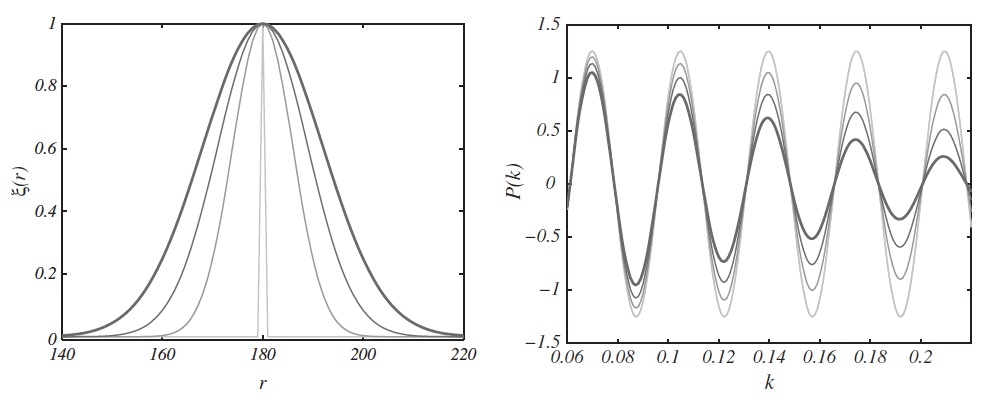
\includegraphics[width=0.9\textwidth]{Images/chapter2/width.png}
       \caption{\small In the left the correlation function and the right the power spectrum. When the width of the peak is increased
       the acoustic oscillation obtained in the power spectrum is damped.    }
       \label{peak}
 \end{figure}
%**********************************************************************************************************************
